\section{Design}
\label{Sec-Design}

Our priority queue exports two operations: \texttt{add()} and \texttt{removeMin()} and is implemented using an underlying skiplist. The elements of the skiplist are buckets associated with keys. For a bucket $b$, the field $b$.key denotes the associated key.
We split the skiplist in two distinct parts. The sequential part, in the beginning of the skiplist, is likely to serve forthcoming \texttt{removeMin()} operations of the priority queue (\texttt{PQ::removeMin()} for short) as well as \texttt{add($v$)} operations of the priority queue (\texttt{PQ:add()} for short) with $v$ small enough (hence expected to be removed soon). The \emph{parallel part}, which complements the sequential part, is likely to serve \texttt{PQ::add($v$)} operations where $v$ is large enough (hence not expected to be removed soon). Either the sequential or the parallel part may become empty.
Both lists are complete skiplists, with (dummy) head buckets called \texttt{headSeq} and \texttt{headPar}, respectively, with key $- \infty$. Both lists also contain (dummy) \texttt{tail} buckets, with key $+ \infty$. We call the last non-dummy bucket of the sequential part \texttt{lastSeq}, which is the logical divisor between parts. Figure~\ref{fig:pqe} shows the design.

\begin{figure}[htb]
\centering
  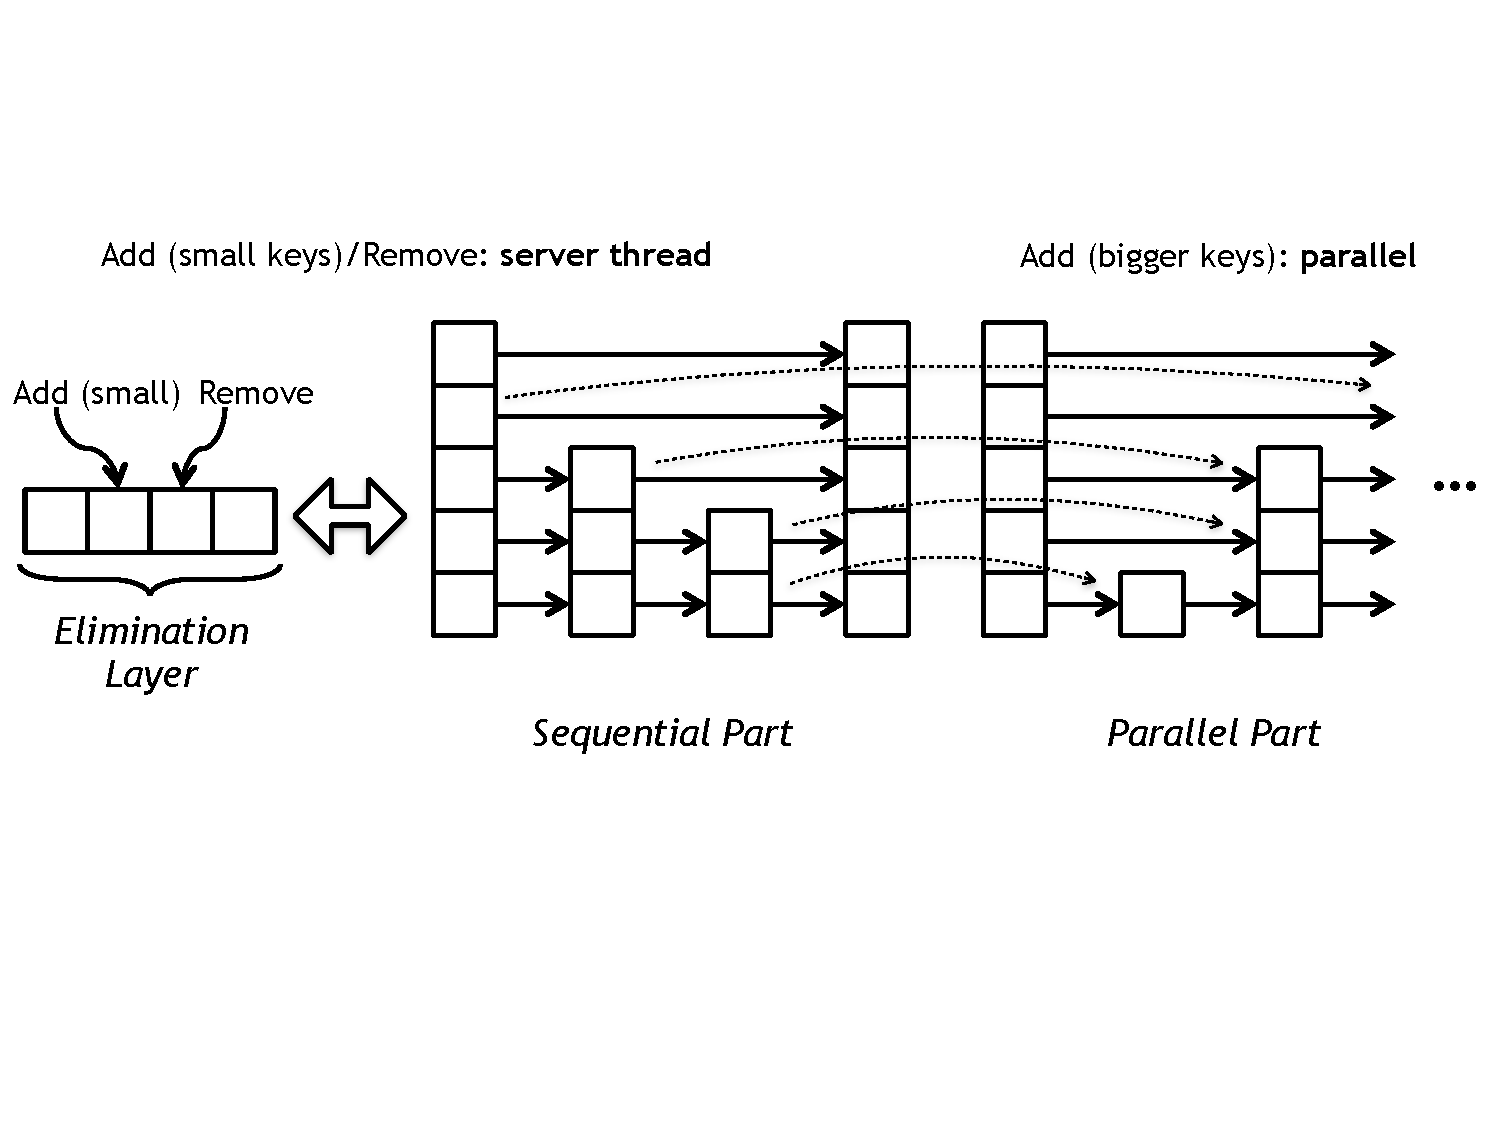
\includegraphics[width=0.9\textwidth]{img/pqe.pdf}
\caption{Skiplist design. An elimination array is used for \texttt{removeMin()}s and \texttt{add()}s with small keys. A dedicated server thread collects the operations that do not eliminate and executes them on the sequential part of the skiplist. Concurrent threads operate on the parallel part, performing \texttt{add()}s with bigger keys. The dotted lines show pointers that would be established if the single skiplist was not divided in two parts.}
\label{fig:pqe}
\end{figure}

%Threads share an \emph{elimination array} (see Sec.~\ref{Sec-Design-Elimination}), operated by a \emph{server thread}, which matches add/remove operations (see Sec.~\ref{Sec-Design-Elimination}) and reduces contention in the sequential part of the skiplist.

When a thread performs a \texttt{PQ::add($v$)}, either (1) $v > \mathtt{lastSeq.key}$, and the thread inserts the value concurrently in the parallel part of the skiplist, calling the \texttt{SL::addPar()} skiplist operation; or (2) $v \le$ \texttt{lastSeq.key}, and the thread tries to perform elimination with a \texttt{PQ::removeMin()} using the elimination array. 
A \texttt{PQ::add($v$)} with $v$ less than the smallest value in the priority queue can immediately eliminate with a \texttt{PQ::removeMin()}, if one is available. A \texttt{PQ::add($v$)} operation with $v$ bigger than \texttt{minValue} (the current minimal key) but smaller than $\mathtt{lastSeq.key}$ lingers in an \emph{elimination array} for some time, waiting to become eligible for elimination or timeout. A \emph{server thread} executes sequentially all operations that fail to eliminate.

This mechanism describes the first elimination algorithm for a priority queue, well integrated with delegation/combining, presented in more detail in Section~\ref{Sec-Design-EliminationCombining}.
Specifically: (1) The scheme harnesses the parallelism of the priority queue \texttt{add()} operations, letting the ones with keys physically distant and large enough (bigger than \texttt{lastSeq.key}) execute in parallel. (2) At the same time, we batch concurrent priority queue \texttt{add()} with small keys and \texttt{removeMin()} operations that timed out in the elimination array, serving such requests quickly through the server thread -- this latter operation simply consumes elements from the sequential part by navigating through elements in its bottom level, merely decreasing counters and moving pointers in the most common situation. While detaching a sequential part is non-negligible cost-wise, a sequential part has the potential to serve multiple removals.

\subsection{Concurrent Skiplist}
\label{Sec-Design-ConcurrentSkiplist}

Our underlying skiplist is operated by the server thread in the sequential part and by concurrently inserting threads with bigger keys in the parallel part.

\textbf{Sequential part.} 
The server calls the skiplist function \texttt{SL::moveHead()} to extract a new sequential part from the parallel part if some \texttt{PQ::removeMin()} operation was requested and the sequential part was empty. 
Conversely, it calls the skiplist function \texttt{SL::chopHead()} to relink the sequential and the parallel parts, forming a completely parallel skiplist, if no \texttt{PQ::removeMin()} operations are being requested for some time.
In \texttt{SL::moveHead()}, we initially determine the elements to be moved to the sequential part. If no elements are found, the server clears the sequential part, otherwise separating the sequential part from the rest of the list, which becomes the parallel part. The number of elements that \texttt{SL::moveHead()} tries to detach to the sequential part adaptively varies between 8 and 65,536. Our policy is simple: if more than N insertions (e.g. N $=$ 1000) occurred in the sequential part since the last \texttt{SL::moveHead()}, we halve the number of elements moved; otherwise, if less than M insertions (e.g. M $=$ 100) were made, we double this number.
After \texttt{SL::moveHead()} executes, a pointer called \texttt{currSeq} indicates the first bucket in the sequential part, and another called \texttt{lastSeq} indicates the final bucket.
The server uses \texttt{SL::addSeq()} and \texttt{SL::removeSeq()} within the sequential part to remove elements or insert elements with small keys (i.e., belonging to the sequential part) that failed to eliminate.
Buckets are not deleted at this time; they are deleted lazily when the whole sequential part gets consumed. A new sequential part can be created by calling \texttt{SL::moveHead()} again.

\textbf{Parallel part.} The skiplist function \texttt{SL::addPar()} inserts elements into the parallel part, and is called by concurrent threads performing \texttt{PQ::add()}. While these insertions are concurrent, the skiplist still relies on a Single-Writer Multi-Readers lock with writer preference for the following purpose. Multiple \texttt{SL::addPar()} operations acquire the lock for reading (executing concurrently), while \texttt{SL::moveHead()} and \texttt{SL::chopHead()} operations acquire the lock for writing. This way, we avoid that \texttt{SL::addPar()} operates on buckets that are currently being moved to the sequential part by \texttt{SL::moveHead()}, or interferes with \texttt{SL::chopHead()}.
Despite the lock, \texttt{SL::addPar()} is not mutually exclusive with the \emph{head-moving operations} (\texttt{SL::moveHead()} and \texttt{SL::chopHead()}). Only the pointer updates (for new buckets) or the counter increment (for existing buckets) must be done in the parallel part (and not have been moved to the sequential part) after we determine the locations of these changes.
Hence, in the \texttt{SL::addPar()} operation, we first try to get a \emph{clean} \texttt{SL::find()}: a \texttt{SL::find()} followed by acquiring the lock for reading, with no intervening head-moving operations. We can tell whether no head-moving operation took place since our lock operations always increases a timestamp variable, checked in the critical section. After a clean \texttt{SL::find()}, now holding the lock, if a bucket corresponding to the key is found, we insert the element in the bucket (incrementing a counter). Otherwise, a new bucket is created, and inserted level by level using \texttt{CAS()} operations. If a \texttt{CAS()} fails in a certain level, we release the lock and retry a clean \texttt{SL::find()}.

Our algorithm differs from the traditional concurrent skiplist insertion algorithms in two ways: (1) we hold a lock to avoid head-moving operations to take place after a clean \texttt{SL::find()}; and (2) if the new bucket is moved out of the parallel section while we insert the element in the upper levels, we stop \texttt{SL::addPar()}, leaving this element with a capped level. This bucket is likely to be soon consumed by a \texttt{SL::removeSeq()} operation, resulting from a \texttt{PQ::removeMin()} operation.

\subsection{Elimination and Combining}
\label{Sec-Design-EliminationCombining}

Elimination allows matching operations to complete without accessing the shared data structure, thus increasing parallelism and scalability. In a priority queue, any \texttt{SL::removeMin()} operation can be eliminated, but only \texttt{SL::add()} operations with values smaller or equal to the current minimum value can be so. If the priority queue is empty, any \texttt{SL::add()} value can be eliminated. 
We used an elimination array similar to the one in the stack elimination algorithm~\cite{Hendler2010a}. Each slot uses 64 bits to pack together a 32-bit value that represents either an opcode or a value to be inserted in the priority queue and a stamp that is unique for each operation. The opcodes are: EMPTY, REMREQ, TAKEN and INPROG. These are special values that cannot be used in the priority queue. All other values are admissible. In our implementation, each thread has a local count of how many operations it performed. This count is combined with the thread ID to obtain a unique stamp for each operation. Overflow was not an issue in our experiments, but if it becomes a problem a different algorithm for associating unique stamps to each operation could be used. The unique stamp is used to ensure linearizability, as explained in Section~\ref{Sec-Linearizability}. All slots are initially empty, marked with the special value EMPTY, and the stamp value is zero. 
  
A \texttt{PQ::removeMin()} thread loops through the elimination array until it finds a request to eliminate with or it finds an empty slot in the array, as described in Algorithm~\ref{Alg-removeMin}.
If it finds a value in the slot, then it must ensure that the stamp is positive, otherwise the value was posted as a response to another thread. The value it finds must be smaller than the current priority queue minimum value. Then, the \texttt{PQ::removeMin()} thread can \texttt{CAS} the slot, which contains both the value and the stamp, and replace it with an indicator that the value was taken (TAKEN, with stamp zero). The thread returns the value found. If instead, the \texttt{PQ::remove()} thread finds an empty slot, it posts a \emph{remove request} (REMREQ), with a unique stamp generated as above. The thread waits until the slot is changed by another thread, having a value with stamp zero. The \texttt{PQ::removeMin()} thread can then return that value. 

\begin{algorithm}[htb]
\caption{PQ::removeMin()}
\label{Alg-removeMin}
\begin{algorithmic}[1]
\While{$\mathbf{true}$}
	\State pos \attr $(id + 1) \% $ ELIM\_SIZE; (value, stamp) \attr elim[pos]
	\If {IsValue(value) \textbf{and} (stamp $> 0$) \textbf{and} (value $\le$ skiplist.minValue))}
	    \If{CAS(elim[pos], (value, stamp), (TAKEN, 0))}
		\State \Return value
	    \EndIf
	\EndIf
	\If {value = EMPTY}
	    \If{CAS(elim[pos], (value, stamp), (REMREQ, uniqueStamp()))}
		\Repeat
		  \State (value, stamp) \attr elim[pos]
		\Until{value $\ne$ REMREQ \textbf{and} value $\ne$ INPROG}
		\State elim[pos] \attr (EMPTY, 0); \Return value
	    \EndIf    
	\EndIf
	\State inc(pos)
\EndWhile
\end{algorithmic}
\end{algorithm}

A \texttt{PQ::add()} thread initially tries to use \texttt{SL::addPar()} to add its value in parallel. A failed attempt to add in parallel indicates that the value should try to eliminate or should be inserted in the sequential part. The \texttt{PQ::add()} thread tries to eliminate by checking through the elimination array for REMREQ indicators. If it finds a remove request, and its value is smaller than the priority queue \texttt{minValue}, it can \texttt{CAS} its value with stamp zero, effectively handing it to another thread. If multiple such attempts fail, the thread changes its behavior: it still tries to perform elimination as above, but as soon as an empty slot is found, it uses a \texttt{CAS} to insert its own value and the current stamp in the slot, waiting for another thread to match the operation (and change the opcode to TAKEN) returning the corresponding value.

The \texttt{PQ::add()} and \texttt{PQ::removeMin()} threads that post a request in an empty slot of the elimination array wait for a matching thread to perform elimination. However, elimination could fail because no matching thread shows up or because the \texttt{PQ::add()} value is never smaller than the priority queue \texttt{minValue}. To ensure that all threads make progress, we use a dedicated \emph{server thread} that collects add and remove requests that fail to eliminate. 
The server thread executes the operations sequentially on the skiplist, calling \texttt{SL::addSeq()} and \texttt{SL::removeSeq()} operations. To ensure linearizability, the server marks a slot that contains an operation it is about to execute as \emph{in progress} (INPROG). Subsequently, it executes the sequential skiplist operation and writes back the response in the elimination slot for the other thread to find it. A state machine showing the possible transitions of a slot in the elimination array is shown in Figure~\ref{fig:transitions}, and the algorithm is described in Algorithm~\ref{Alg-Execute}.

\begin{algorithm}[htb]
\caption{Server::execute()}
\label{Alg-Execute}
\begin{algorithmic}[1]
\While{$\mathbf{true}$}
  \For{$i$: 1 $\rightarrow$ ELIM\_SIZE}
	\State (value, stamp) \attr elim[i]
	\If{value = REMREQ}
	    \If{CAS(elim[i], (value, stamp), (INPROG, 0))}
		\State min \attr skiplist.removeSeq(); elim[i] \attr (min, 0)
	    \EndIf
	\EndIf
	\If {IsValue(value) \textbf{and} (stamp $> 0$)}
	    \If{CAS(elim[i], (value, stamp), (INPROG, 0))}
		\State skiplist.addSeq(value); elim[i] \attr (TAKEN, 0)
	    \EndIf    
	\EndIf
  \EndFor
\EndWhile
\end{algorithmic}
\end{algorithm}

\begin{figure}
  \centering
	  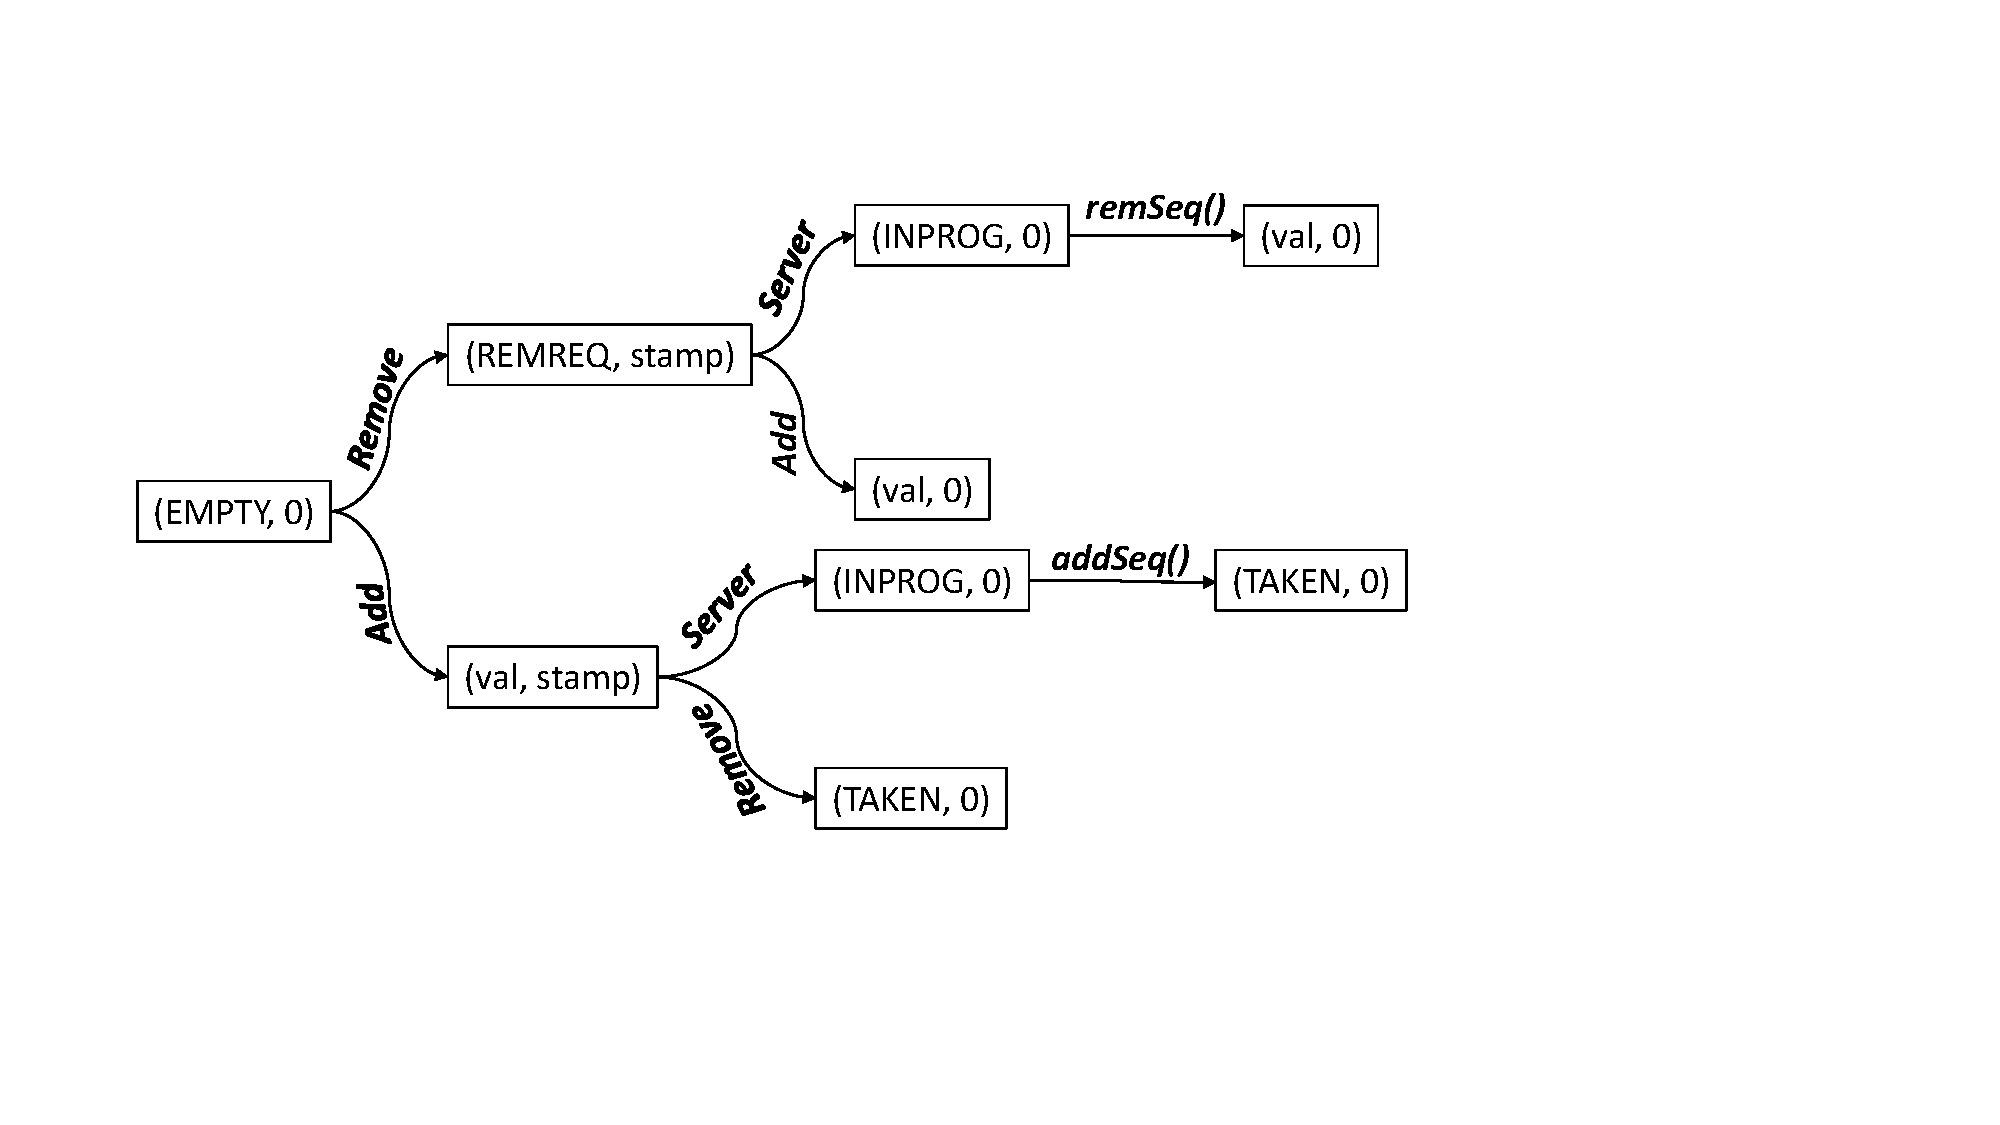
\includegraphics[width=0.75\textwidth]{img/combining-state.pdf}
\caption{Transitions of a slot in the elimination array.}
\label{fig:transitions}
\end{figure}
